\section{Call option price in the Black \& Scholes model}\lesson{12}{03/04/2020}
Start with the risk neutral dynamics of the assets:
\begin{equation}
    \frac{\dd S}{S} = \mu\dd t + \sigma \dd W^{\Qmeas}, \qquad \frac{\dd B}{B} = r\dd t.
\end{equation}
The call option payoff is given by
\begin{equation}
    \call_T = (S_T - K)^+ = \pay_T.
\end{equation}
Let's consider the case in which $t=0$, so that in the price of the call we have to compute an unconditional expected value:
\begin{equation}
    price_0(\call) = e^{-rt}\mathbb{E}^{\Qmeas}[(S_T-K)^+].
\end{equation}
We know that, under $\Qmeas$, $S_T$ is a Brownian motion:
\begin{equation}
    S_T = S_0\exp{\left(r-\dfrac{\sigma^2}{2}\right)T+\sigma W_T^{\Qmeas}},
\end{equation}
where $W_T^{\Qmeas}=\sqrt{T}\mathcal{N}(0,1)$. So, we have to compute:
\begin{equation}
    price_0(\call) = e^{-rt}\int_{\mathbb{R}}\left(S_0\exp{\left(r-\dfrac{\sigma^2}{2}\right)T+\sigma \sqrt{T}y}-K\right)^+\frac{1}{\sqrt{2\pi}}e^{-\frac{y^2}{2}}\dd y.
\end{equation}
In order to remove the non-linearity given by the positive part, we study the sign of the expression:
\begin{align}
    S_0\exp{\left(r-\dfrac{\sigma^2}{2}\right)T+\sigma \sqrt{T}y}-K \ge 0.
\end{align}
If we take the logarithm, we get:
\begin{equation*}
    \left(r-\dfrac{\sigma^2}{2}\right)T+\sigma \sqrt{T}y \ge \ln\frac{K}{S_0},
\end{equation*}
\begin{equation*}
    y \ge \dfrac{\ln\frac{K}{S_0} - \left(r-\frac{\sigma^2}{2}\right)T}{\sigma\sqrt{T}} \equiv \hat{y}.
\end{equation*}
So, if $y\ge\hat{y}$ we can remove the positive part:
\begin{align}
    \notag price_0(\call) &= S_0\cancel{e^{-rT}}\int_{\hat{y}}^{+\infty}\exp{\left(\cancel{r}-\dfrac{\sigma^2}{2}\right)T+\sigma\sqrt{T}y}\frac{1}{\sqrt{2\pi}}e^{-\frac{y^2}{2}}\dd y - \\
    &\qquad
    \notag - Ke^{-rT}\int_{\hat{y}}^{+\infty}\frac{1}{\sqrt{2\pi}}e^{-\frac{y^2}{2}}\dd y \\
    \overset{(a)}&{=}
    \notag \frac{S_0}{\sqrt{2\pi}}\int_{\hat{y}}^{+\infty}\exp{-\dfrac{\sigma^2}{2}T+\sigma\sqrt{T}y-\frac{y^2}{2}}\dd y - Ke^{-rt}\Phi(-\hat{y}) \\
    \overset{(b)}&{=}
    \notag \frac{S_0}{\sqrt{2\pi}}\int_{\hat{y}}^{+\infty}\exp{-\dfrac{1}{2}(y-\sigma\sqrt{T})^2}\dd y - Ke^{-rt}\Phi(-\hat{y}) \\
    \overset{(c)}&{=}
    \notag \frac{S_0}{\sqrt{2\pi}}\int_{\hat{y}-\sigma\sqrt{T}}^{+\infty}e^{-\dfrac{z^2}{2}}\dd z - Ke^{-rt}\Phi(-\hat{y}) \\
    &=
    S_0\Phi(\sigma\sqrt{T}-\hat{y})-Ke^{-rt}\Phi(-\hat{y}),
\end{align}
where:
\begin{itemize}
    \item in (a) we used the cumulative distribution function $$\Phi(x)=\int_{-\infty}^x \frac{1}{\sqrt{2\pi}}e^{-\frac{y^2}{2}}\dd y;$$
    \item in (b) we recognized that the argument of the exponent is a square expansion;
    \item in (c) we introduced the change of variable $z=y-\sigma\sqrt{T}$, $\dd z = \dd y$.
\end{itemize}
So we end up with the following Black \& Scholes formula:
\begin{equation}
    price_0(\call) = S_0\Phi(d_1)-Ke^{-rt}\Phi(d_2),
\end{equation}
where
\begin{equation}
    d_1 = \dfrac{\ln\frac{S_0}{K} + \left(r+\frac{\sigma^2}{2}\right)T}{\sigma\sqrt{T}}, \qquad d_2 = d_1 - \sigma\sqrt{T}.
\end{equation}
What about the case in which $t\in(0,T)$? In this case
\begin{equation}
    price_t(\call) = e^{-rt}\mathbb{E}_t^{\Qmeas}[(S_T-K)^+]
\end{equation}
and
\begin{align}
    \notag S_T &= S_0\exp{\left(r-\dfrac{\sigma^2}{2}\right)(T-t)+\sigma (W_T^{\Qmeas}-W_t^{\Qmeas})} \\
    &=
    S_0\exp{\left(r-\dfrac{\sigma^2}{2}\right)(T-t)+\sigma\sqrt{T-t}\mathcal{N}(0,1)}.
\end{align}
Now $S_t$ is measurable and $(W_T^{\Qmeas}-W_t^{\Qmeas})$ is a gaussian random variable independent of the information available at time $t$, $\mathcal{F}_t $. This independence allows us to eliminate the conditioning in the expected value. So we only have to repeat the procedure substituting $S_0\to S_t$ and $T\to T-t$. In the end we arrive at the following Black \& Scholes formula (1973):
\begin{equation}\label{B&S}
    price_t(\call) = S_t\Phi(d_1)-Ke^{-r(T-t)}\Phi(d_2),
\end{equation}
where
\begin{equation}\label{d}
    d_1 = \dfrac{\ln\frac{S_t}{K} + \left(r+\frac{\sigma^2}{2}\right)(T-t)}{\sigma\sqrt{T-t}}, \qquad d_2 = d_1 - \sigma\sqrt{T-t}.
\end{equation}
At the time, no financial journal accepted to publish this result. In order to understand the reason, we consider an example.
\begin{example}{}{}{}
    Suppose we have two assets, Alitalia and Facebook, and that the volatility and the initial price are the same, $\sigma_A = \sigma_F$ and $S_0^A = S_0^F$. Let's consider a call option at the money ($S_0=K$) with maturity $T=1$ year for both of them. Facebook's shares price is expected to increase, while Alitalia's one is expected to decrease. So, the payoffs will be
    \begin{equation*}
        (S_T^F-K)^+ > 0, \qquad (S_T^A-K)^+ = 0
    \end{equation*}
    So, it is reasonable to assume that
    \begin{equation*}
        price^A_t(\call) < price^F_t(\call)
    \end{equation*}
    The problem is that we know that all the prices satisfy the PDE, which has solution \eqref{B&S}. But \eqref{B&S} contains no information about the drift, because it is written in terms of the risk neutral probability measure. So, if the two assets share the same parameters (volatility, initial price and maturity) they will have the same price, regardless their historical behavior.
    \begin{equation*}
        price^A_t(\call) = price^F_t(\call)
    \end{equation*}
    This is completely counter-intuitive, and this is why no journal accepted to publish the paper by Black and Scholes. However, even if the academic community did not accept this result\footnote{In the end, the paper was published in the \emph{Journal of Political Economy}, which is not a quantitative journal.}, traders were already using it in their calculators.
\end{example}

\section{The Greeks}
Each Greek letter measures a different dimension of the risk in an option position. The aim of a trader is to manage the Greeks so that all risks are acceptable.

\subsection{Delta}
The most important Greek is the $\Delta$, which represents the sensitivity of the option price (given by the B\&S formula) with respect to the price of the underlying asset:
\begin{equation}\label{apparentlywrong}
    \Delta = \pdv{price}{S} = \Phi(d_1).
\end{equation}
Apparently, this differentiation is not correct, because inside $d_1$ there is a dependence of $S$, as we can see in \eqref{d}. The correct one should be:
\begin{equation}
    \Delta = \pdv{price}{S} = \Phi(d_1) + S_t\pdv{\Phi(d_1)}{S} - Ke^{-r(t-T)}\pdv{\Phi(d_2)}{S}.
\end{equation}
Nevertheless, eq. \eqref{apparentlywrong} is correct. Let's prove it. Recall that
\begin{equation*}
    \Phi(x) = \int_{-\infty}^x\dfrac{e^{-\frac{y^2}{2}}}{\sqrt{2\pi}}\,\dd y.
\end{equation*}
In order to compute the derivative of this integral we use the Lebesgue formula, where we can have the dependence of a parameter (even in the extremes of integration):
\begin{equation}
    \dv{t} \int_{\alpha(t)}^{\beta(t)}f(x,t)\,\dd x = \beta'(t)f(\beta(t),t)-\alpha'(t)f(\alpha(t),t) + \int_{\alpha(t)}^{\beta(t)}\pdv{f(x,t)}{t}\,\dd x.
\end{equation}
In our particular case, we have:
\begin{align}
    \dv{\Phi(d_1)}{S} = \dv{S}\int_{-\infty}^{d_1(S)}\dfrac{e^{-\frac{y^2}{2}}}{\sqrt{2\pi}}\,\dd y
    = d_1'(S)\dfrac{e^{-\frac{d_1^2}{2}}}{\sqrt{2\pi}}
    = \dfrac{1}{S_t\sigma\sqrt{T-t}}\dfrac{e^{-\frac{d_1^2}{2}}}{\sqrt{2\pi}},
\end{align}
\begin{align}
    \dv{\Phi(d_2)}{S} = \dv{S}\int_{-\infty}^{d_2(S)}\dfrac{e^{-\frac{y^2}{2}}}{\sqrt{2\pi}}\,\dd y
    = d_2'(S)\dfrac{e^{-\frac{d_2^2}{2}}}{\sqrt{2\pi}}
    = \dfrac{1}{S_t\sigma\sqrt{T-t}}\dfrac{e^{-\frac{d_2^2}{2}}}{\sqrt{2\pi}},
\end{align}
and
\begin{align*}
    \Delta_t &= \Phi(d_1) + S_t\dfrac{1}{S_t\sigma\sqrt{T-t}}\dfrac{e^{-\frac{d_1^2}{2}}}{\sqrt{2\pi}} - Ke^{-r(T-t)}\dfrac{1}{S_t\sigma\sqrt{T-t}}\dfrac{e^{-\frac{d_2^2}{2}}}{\sqrt{2\pi}}\\
    &=
    \Phi(d_1) + \dfrac{1}{S_t\sigma\sqrt{T-t}\sqrt{2\pi}}\left(S_te^{-\frac{d_1^2}{2}} - Ke^{-r(T-t)}e^{-\frac{d_2^2}{2}}\right)\\
    \overset{(a)}&{=}
    \Phi(d_1) + \dfrac{e^{-\frac{d_2^2}{2}}}{S_t\sigma\sqrt{T-t}\sqrt{2\pi}}\left(S_te^{-\frac{\sigma^2}{2}(T-t)-d_2\sigma(T-t)} - Ke^{-r(T-t)}\right)\\
    \overset{(b)}&{=}
    \Phi(d_1) + \dfrac{e^{-\frac{d_2^2}{2}}}{S_t\sigma\sqrt{T-t}\sqrt{2\pi}}\left(S_te^{\cancel{-\frac{\sigma^2}{2}(T-t)}-\ln\frac{S_t}{K}-\left(r-\cancel{\frac{\sigma^2}{2}}\right)(T-t)} - Ke^{-r(T-t)}\right)\\
    &=
    \Phi(d_1) + \dfrac{e^{-\frac{d_2^2}{2}}}{S_t\sigma\sqrt{T-t}\sqrt{2\pi}}\left(S_te^{-\ln\frac{S_t}{K}-r(T-t)} - Ke^{-r(T-t)}\right) \\
    &=
    \Phi(d_1) + \dfrac{e^{-\frac{d_2^2}{2}-r(T-t)}}{S_t\sigma\sqrt{T-t}\sqrt{2\pi}}\left(S_t \frac{K}{S_t} - K\right) \\
    &=
    \Phi(d_1),
\end{align*}
where in (a) we used the fact that
\begin{align*}
    d_1 = d_2 + \sigma\sqrt{T-t} &\qquad\Rightarrow\qquad d_1^2 = d_2^2 - \sigma^2(T-t) + 2d_2\sigma\sqrt{T-t} \\
    &\qquad\Rightarrow\qquad
    -\frac{1}{2} d_1^2 = -\frac{1}{2} d_2^2 - -\frac{\sigma^2}{2}(T-t) - d_2\sigma\sqrt{T-t}
\end{align*}
and in (b) we used the fact that
\begin{equation*}
    d_2\sigma\sqrt{T-t} = \ln\frac{S_t}{K}+\left(r-\frac{\sigma^2}{2}\right).
\end{equation*}
So, the number of shares we have to get in our portfolio in order to replicate the payoff at the end is $\Phi(d_1)$. \\
The call payoff is equal to zero until $K$ and then it is a straight line with slope $45^\circ$. Being the call price a double derivable function, it must be a smooth function which is very close to zero when the underlying is very low and reaches the behavior of the straight line when the underlying is very big (see Figure \ref{fig:priced}).
\begin{figure}[htp]
    \centering
    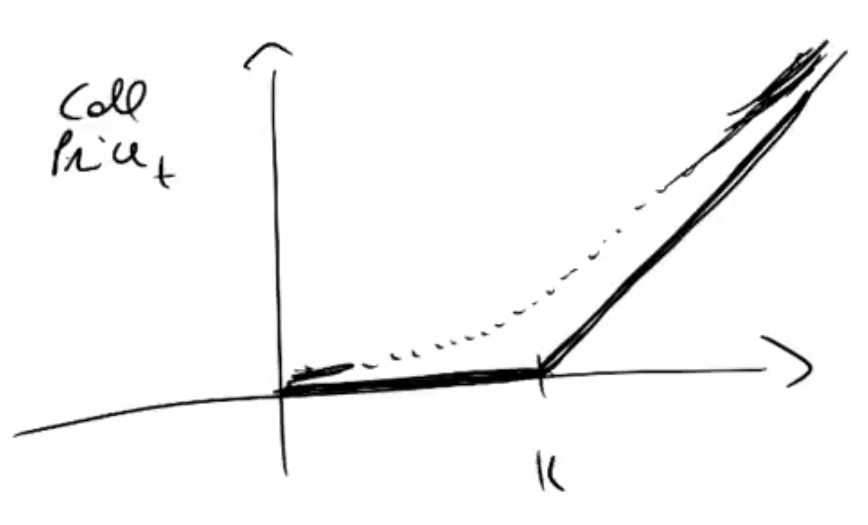
\includegraphics[scale=0.3]{fig/tmp/fig12.png}
    \caption{$\Phi(d_1)$ for call payoff.}
    \label{fig:priced}
\end{figure}
When we take its derivative with respect to $S$, i.e. the $\Delta$, we obtain the cumulative gaussian density (see Figure \ref{fig:delta}).
\begin{figure}[htp]
    \centering
    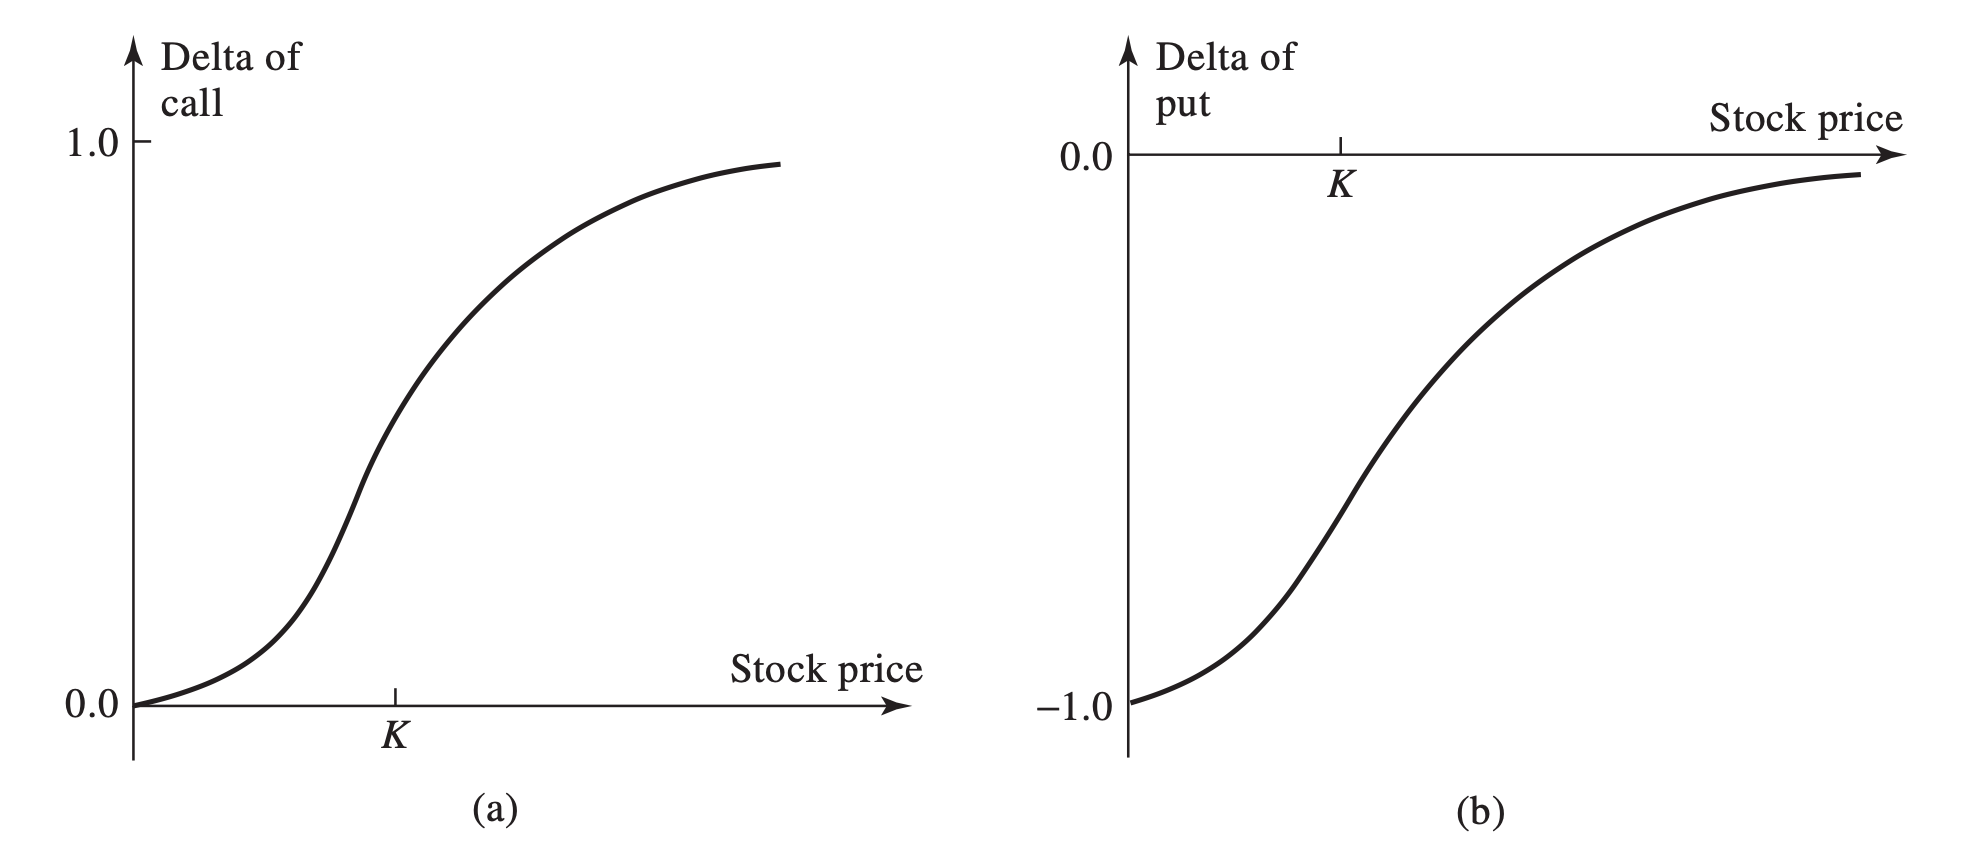
\includegraphics[scale=0.2]{fig/tmp/fig13.png}
    \caption{Variation of delta with stock price for (a) a call option and (b) a put option on a non-dividend-paying stock.}
    \label{fig:delta}
\end{figure}
The financial intuition is the following. When the underlying is less than the strike we are out of the money and there is no need to keep it in our portfolio. On the other hand, if the underlying is greater than the strike we are in the money and in order to construct the payoff for our long counterpart we have to hold a great amount of underlying (almost 1). The problem arises around the strike $K$, because for small fluctuations around $K$ there can be huge changes in the hedging portfolio.\\
So, hedging is more irregular than pricing. This is due to the fact that pricing involves an expectation, which is an integral that increases regularity. On the contrary, by deriving we loose regularity.\\
\\
